Confiabilidade e disponibilidade são características altamente desejáveis em sistemas de computação, pois a humanidade depende cada vez mais de sistemas automatizados e informatizados para a realização de suas tarefas diárias. Dentre estes estão sistemas críticos, como sistemas que envolvam transações financeiras ou o software controlador de um avião onde, por exemplo, falhas podem causar prejuízo financeiro e/ou perda de vidas.

Os computadores (hardware + software) são, provavelmente, os sistemas mais complexos já inventados pelo homem. A complexidade das peças de hardware segue em constante crescimento, o que gera a possibilidade de inserção de defeitos em várias etapas do desenvolvimento, desde o nível elétrico até, por exemplo, bugs nos algoritmos de predição implementados fisicamente nos processadores. A área de software é ainda mais complexa e, por isso, ainda mais propensa a falhas. Até mesmo o ônibus espacial (\emph{Space Shuttle}) da NASA~\cite{BonacheaOnline}, desenvolvido com as mais cuidadosas tecnologias apresentou \emph{bugs} no código de seu sistema, podendo resultar em uma catástrofe. Podemos extrapolar estas situações e afirmar que falhas são inevitáveis em computadores. Contudo, as consequências dessas falhas podem ser contornadas ou, ao menos, minimizadas, caso o design do software seja preparado para lidar com falhas que possam vir a ocorrer no sistema.

É notável o crescimento em confiabilidade na área de hardware, onde vimos uma grande cultura de tolerância a falhas se formar, desde o tempo dos inseguros \emph{mainframes} a vávula, cujos proprietários sofriam rotineiramente com falhas de diversas origens, até os robustos \emph{laptops} e \emph{smartphones} que temos hoje para computação pessoal. Na área de software, por outro lado, os processos de desenvolvimento e os produtos estão cada vez mais complexos e apresentando cada vez mais \emph{bugs}. Uma vez que esses \emph{bugs} são quase inevitáveis, mecanismos de tolerância a falhas se tornam obrigatórios em sistemas onde a confiabilidade e disponibilidade é imprescindível.

Os conceitos apresentados ao longo dessa seção servem como base para melhor compreendermos as técnicas básicas de tolerância a falhas e as sutis variações dos problemas e soluções que aparecem neste sentido em ambiente de computação ubíqua.

\subsection{Falhas, erros e defeitos} % (fold)
\label{sub:falhas_erros_e_defeitos}

Com frequência usamos as palavras ``falha'', ``erro'' e ``defeito'' como sinônimos para designar problemas que fazem um módulo de software ou hardware funcionar de forma indevida. Contudo, na área de tolerância a falhas faz-se uma distinção entre estes três termos. Diversos autores da área possuem definições sutilmente diferentes para esses termos, e as definições que usaremos aqui foram retiradas de~\cite{koren2007fault}.

Uma \textbf{falha}, do inglês \emph{fault} (também traduzido como \textbf{falta}), ou \textbf{defeito} (\emph{failure}) pode ser algum problema diretamente no hardware ou algum \emph{bug} na programação do software. Já o \textbf{erro} é uma manifestação de uma falha.

Por exemplo, considere um circuito que faz a soma de dois números binários, porém com um dos bits de saída preso em $0$ (zero), independente do resultado da soma dos operandos. Este defeito ou falha no hardware só gerará um erro quando a soma dos operandos resultar em um valor em que aquele bit específico da saída não seria igual a zero. Outro exemplo, na área de software, é uma linha \emph{condicional} de código mal programada, a qual pode eventualmente acessar uma área de memória inválida. Esta falha de programação só irá gerar um erro quando, em tempo de execução, o programa executar esta linha de código e acessar alguma área de memória inválida.

Falhas e erros podem, também, se propagar em um sistema. Por exemplo, o somador defeituoso pode passar um resultado errado para outros componentes que usarão sua saída como dado de entrada, fazendo até mesmo com que erros sejam capturados em módulos não defeituosos. Programadores e projetistas devem prever \textbf{zonas de contenção} em seus sistemas para impedir que erros e defeitos se propaguem para outras partes do sistema. Por exemplo, um \emph{chip} queimado pode desligar outros componentes de hardware ligados a ele, a menos que a energia seja fornecida a cada componente de forma individual ou haja um \emph{chip} ``estepe'' que é ativado em caso de falha do \emph{chip} ``titular''. Ainda, vários chips podem operar simultaneamente sobre o mesmo conjunto de dados, com suas saídas sendo passadas a um componente que faz uma votação sobre as respostas. Estratégias desse tipo fazem com que falhas em um componente específico não se propaguem pelo restante do sistema.

% subsection falhas_erros_e_defeitos (end)

\subsection{Classificação de falhas de hardware} % (fold)
\label{sub:classificacao}

Falhas de hardware podem ser classificadas sob diversos aspectos. Em relação a seu tempo de duração, estas podem ser classificadas em falhas \emph{permanentes}, \emph{transientes}, ou \emph{intermitentes}. \emph{Falhas permanentes} são aquelas onde um componente falha e não volta a funcionar, como um LED que queima, por exemplo. \emph{Falhas transientes} são aquelas onde um certo componente apresenta funcionamento defeituoso e após algum tempo volta a funcionar correta e plenamente. Um exemplo pode ser uma célula de memória que tem seu valor alterado por uma interferência magnética, porém sua funcionalidade segue intacta: uma reescrita na memória soluciona a falha ocorrida. \emph{Falhas intermitentes} são aquelas que não desaparecem por completo, onde um componente apresenta determinada falha com uma certa periodicidade. Uma falha intermitente apresenta períodos de quiescência, onde o componente funciona normalmente, e períodos de atividade, onde o componente falha. Um exemplo pode ser uma corrente de energia instável.

Falhas de hardware podem ser também classificadas em \emph{benignas} e \emph{maliciosas}. Uma falha \emph{benigna} é aquela que simplesmente faz o componente parar de funcionar, o que é relativamente fácil de tratar. No entanto, um componente poder seguir funcionando sem problemas aparentes e gerando resultados incorretos. Este tipo de falha é mais difícil de identificar e pode gerar problemas delicados. Podemos pensar, por exemplo, em um avião cujo sensor de altitute mede um valor incorreto que é entregue no mostrador do piloto, o qual depende da corretude desta informação para guiar o avião. Este segundo tipo de falhas chamamos de \emph{maliciosa} (ou \emph{bizantina}).
% subsection classificacao (end)

\subsection{Redundância} % (fold)
\label{sub:redundancia}

Praticamente todas as técnicas de tolerância a falhas envolvem algum tipo de redundância. Por redundância entende-se o fato de existir mais de um componente (de software ou hardware) no sistema fornecendo a mesma funcionalidade. Em geral, estas técnicas de tolerância a falhas consistem de mecanismos de autogerenciamento dos componentes redundantes.

Existem basicamente quatro tipos de redundâncias: redundância de \emph{hardware}, \emph{software}, \emph{informação} e \emph{tempo}. Falhas de hardware geralmente são prevenidas com redundância de hardware, informação e tempo, enquanto falhas de software são prevenidas com redundância de software.

\emph{Redundância de hardware} é geralmente obtida por peças de hardware extra que simplesmente detectam a falha de outro componente de hardware ou sobrescreve o efeito de sua falha. Esta redundância de hardware pode ser \emph{estática}, quando diversos componentes iguais, e.g. processadores, funcionam simultaneamente para realizar a mesma função, mascarando imediatamente uma falha, ou \emph{dinâmica}, quando um componente ``estepe'' é ativado quando outro falha, cada qual com seus prós e contras. Uma combinação destas duas técnicas é possível, resultando em uma \emph{redundância híbrida de hardware}.

A técnica mais conhecida que envolve \emph{redundância de informação} é, sem dúvida, códigos para detecção e correção de erros (e.g., \emph{checksums}). Nesta técnica, \emph{bits} extras são adicionados aos dados originais de forma que erros em uma transmissão de dados possam ser detectados e, até mesmo, corrigidos. Códigos de detecção e correção de erros têm uma aplicação essencial na proteção das transmissão de dados por canais ruidosos, seja em uma rede local ou na internet. Se o código adicional é capaz apenas de identificar e não corrigir erros, estes precisarão ser retransmitidos, resultando em uma \emph{redundância de tempo}. Ainda, se uma falha permanente de um link tornar um nó inalcançável, deve-se usar links redundantes, isto é, \emph{redundância de hardware}.

Como a maioria das falhas de hardware são transientes, é improvável que uma re-execução da mesma computação no mesmo hardware irá ser acometida pela mesma falha. Assim, pode-se aplicar \emph{redundância de tempo} pela simples re-execução da computação em questão. Redundância de tempo, em geral, não gera custos significativos em hardware e software, porém acarreta em uma grande perda de desempenho.

\emph{Redundância de software} engloba técnicas para proteger o sistema principalmente de \emph{bugs} no software. Alcançar este nível pode ser custoso: uma técnica simples é ter duas ou mais versões das funções mais importantes do sistema (de preferência, implementadas por times diferentes). A premissa é de que é pouco provável que ambos os códigos irão gerar erros de execução para as mesmas entradas. As versões secundárias podem implementar algoritmos menos precisos e menos complexos (e, consequentemente, menos propensos a falhas) para produzirem resultados aceitáveis em caso de falha do primeiro. Assim como na redundância de hardware, as versões implementadas pode ser executadas paralelamente (necessitando, também, de hardware redundante) ou sequencialmente (necessitando tempo extra e/ou redundância de tempo) em caso de falha um dos módulos módulo de software

\subsection{Dependabilidade} % (fold)
\label{sub:dependabilidade}

O objetivo da tolerância a falhas é aumentar a dependabilidade dos sistemas. Este termo é uma tradução literal do termo original em inglês, \emph{dependability}, o qual indica um grau de qualidade do serviço fornecido por um sistema qualquer e o grau de confiança que os usuários possuem nesse sistema.

O conjunto de atributos que formam o conceito de dependabilidade são unidades que podem ser medidas em um sistema. Estes atributos são confiabilidade, disponibilidade, segurança de funcionamento (\emph{safety}), segurança de acesso (\emph{security}), mantenablidade, testabilidade e comprometimento com o desempenho. Com excessão deste último, os demais atributos estão sumarizaddos na tabela~\ref{tab:dependabilidade}.

\begin{table*}
\begin{center}
\caption{Resumo dos atributos de dependabilidade.}\label{tab:dependabilidade}

	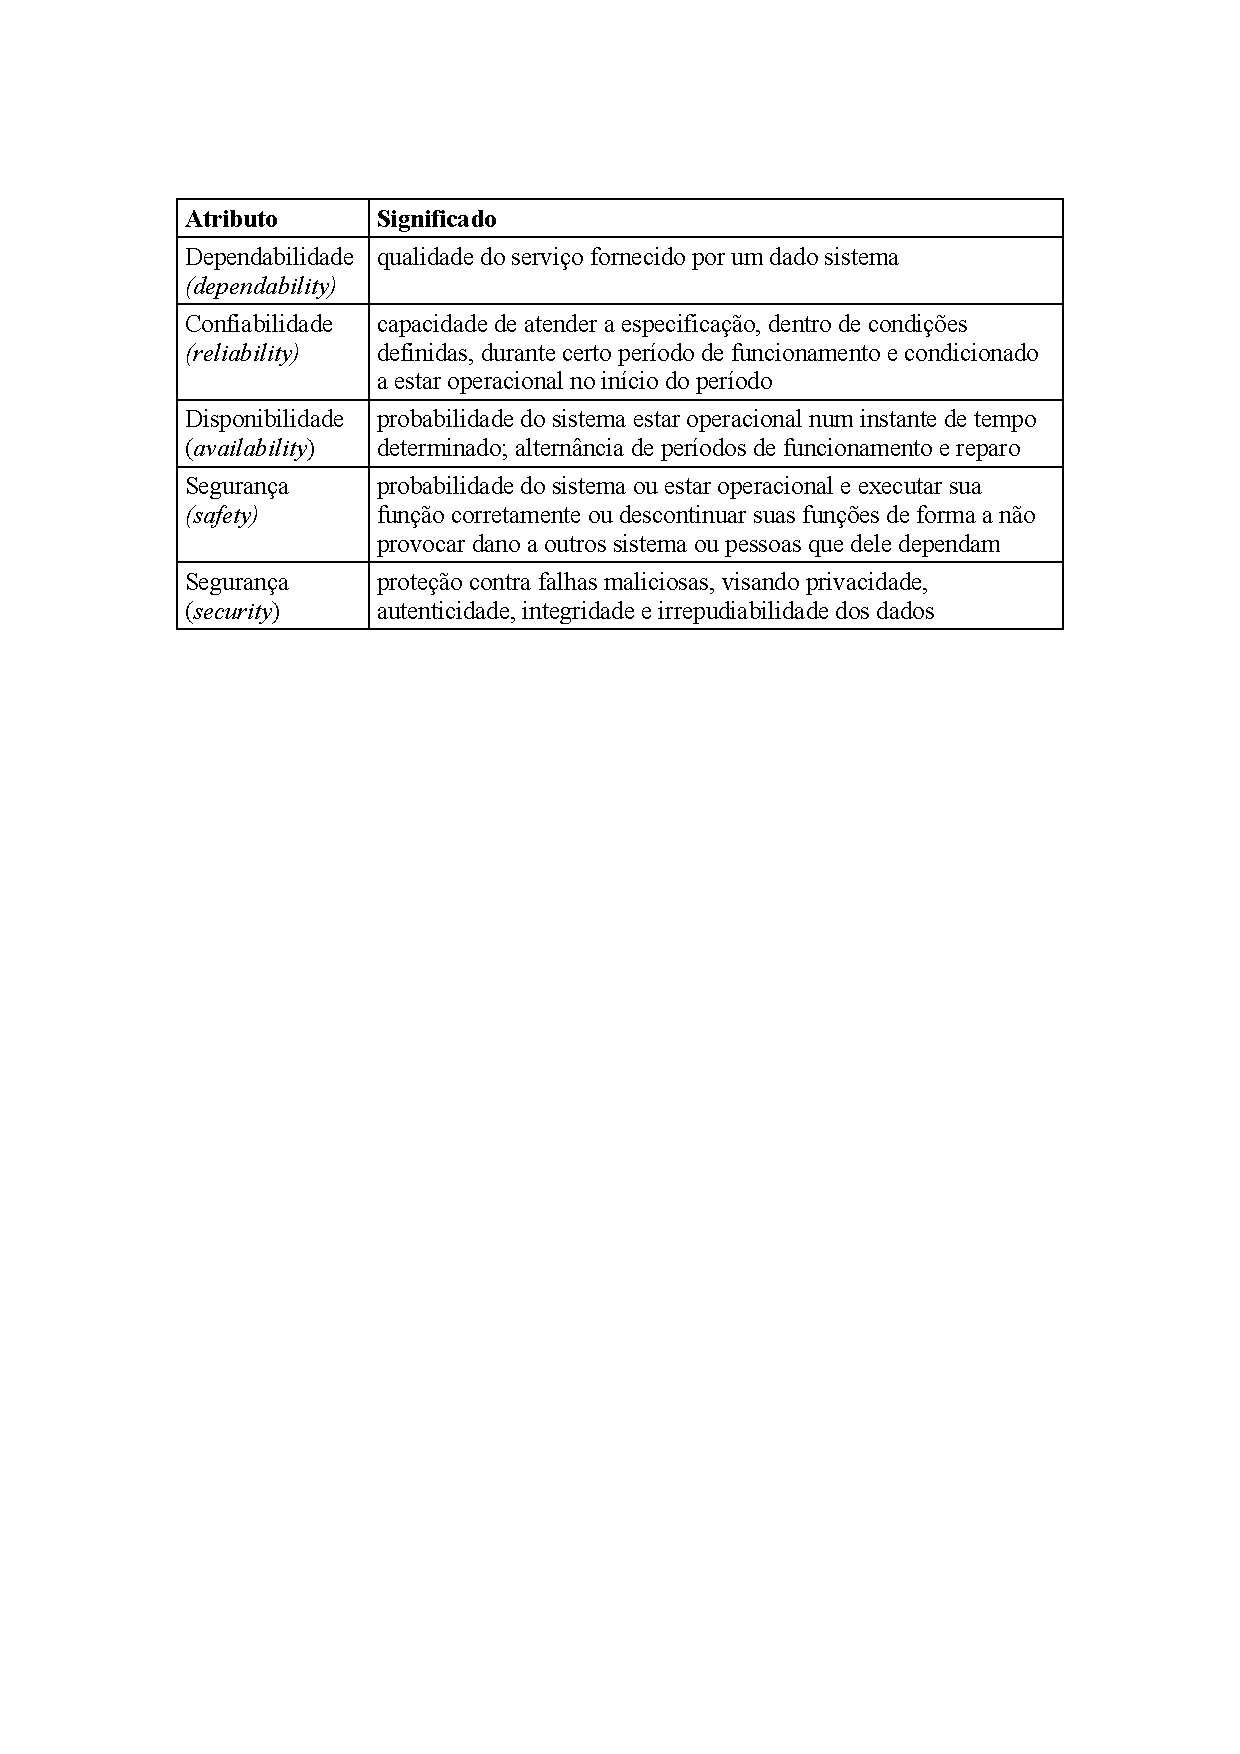
\includegraphics[height=3in]{figuras/tabela_weber.pdf}

\end{center}
\end{table*}
% subsection dependabilidade (end)